\documentclass[final]{siamltexmm}
\documentclass[10pt,a4paper]{article}

\usepackage{graphicx}
\usepackage{algorithm}
\usepackage{algorithmic}

% \usepackage[demo]{graphicx}
% \usepackage{subfig}

\newcommand{\pe}{\psi}
\def\d{\delta} 
\def\ds{\displaystyle} 
\def\e{{\epsilon}} 
\def\eb{\bar{\eta}}  
\def\enorm#1{\|#1\|_2} 
\def\Fp{F^\prime}  
\def\fishpack{{FISHPACK}} 
\def\fortran{{FORTRAN}} 
\def\gmres{{GMRES}} 
\def\gmresm{{\rm GMRES($m$)}} 
\def\Kc{{\cal K}} 
\def\norm#1{\|#1\|} 
\def\wb{{\bar w}} 
\def\zb{{\bar z}} 

% some definitions of bold math italics to make typing easier.
% They are used in the corollary.

\def\bfE{\mbox{\boldmath$E$}}
\def\bfG{\mbox{\boldmath$G$}}

\title{Independent Study}
\author{Yun-shao Sung\thanks{\tt yss265@nyu.edu} }

\begin{document}
\maketitle

\begin{abstract}
This is independent study mid-way report
\end{abstract}

\pagestyle{myheadings}
\thispagestyle{plain}

\section{Abstract}
There are many approaches to understand the structure of music, and this is a project applying spectral graph theory with Laplacian formula to analyze repeated patterns in musical recordings. Starting with low-dimensional encoding of repeating structure, hierarchical relationship among repeating components will be built by changing number of eigenvectors. Further works for this project will include Neural Network and back-propagation to apply thie technique to analyze the structure of wide variety of musics.

\\
\section{Introduction}
Hi2!

\\
\section{Baseline Approach}
Here is the baseline approach which can be roughtly divided into two parts: the first part is constructing \textit{sequence-augmented affinity matrix A} from \textit{symmetric matrix R} of the feature similarity at each time points, and the second part is to construct symmetric normalized Laplacian matrix and obtain the top $m$ eigenvectors with the top $m$ smallest eigenvalues, and then perform k-means for boundary detection. The high level pseudocode is described in Algorithm 1.

\begin{algorithm}[htb]
  \caption{Baseline Approach}
  \SetKwInOut{Input: }{number of top $m$ smallest eigenvalues}
  \label{algo:SC}
\begin{algorithmic}[1]
  \STATE M = getSymmetricMatrix() //to get affinity matrix
  \STATE L = scipy.sparse.csgraph.laplacian() //to get symmetric normalized Laplacian matrix
  \STATE eigVals, eigVecs = np.linalg.eig(L)
  \STATE Y = getMthSmallest(eigVals, eigVecs, m)
  \STATE return boundaryDetection(Y)
\end{algorithmic}
\end{algorithm}


\subsection{Symmetric and Laplacian Matrix}
Initially symmetric matrix is constructed manually, and the symmetric properity is ensured by checking $m == m^T$. The following symmetric normalized Laplacian L is defined as:
\begin{equation}
L = I - D^{-1/2}AD^{-1/2}
\end{equation}
The properity of symmetric is important as it shows the correlation between time $i$ and $j$ which is an undirected graph, and the proterity is important to hold to make sure the eigenvectors calculated from Laplacian matrix is done correctly. Figure 3.1 shows the example of symmetrix matrix and its corresponding top-10 eignevectors, and method is implemented from Algoritm 1.

\begin{figure}[H]
\centering
\begin{subfigure}
  \begin{tabular}{c}
  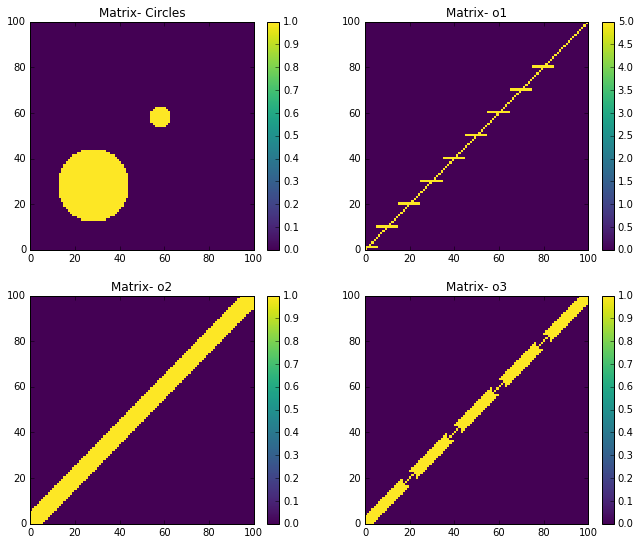
\includegraphics[width=50mm]{./figure/similarityMatrix.png}
  \end{tabular}{}
\end{subfigure}
  \begin{tabular}{c}
  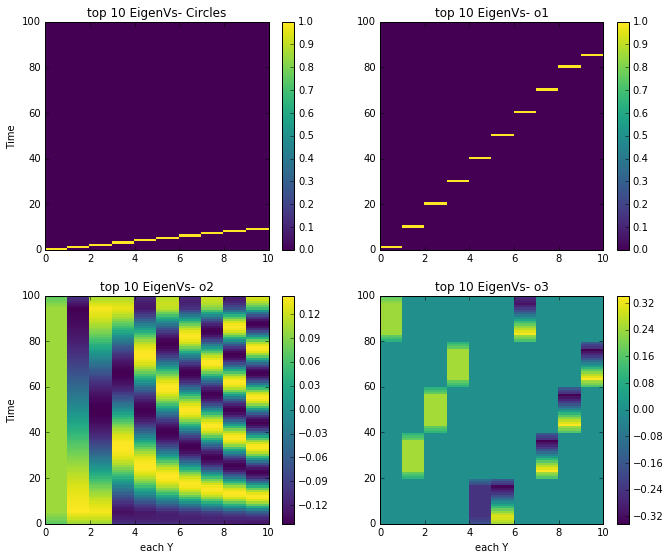
\includegraphics[width=50mm]{./figure/similarityMatrix_eigens.png}
  \end{tabular}{}
\begin{subfigure}
\end{subfigure}
\caption{Symmetric matrix and eigen vectors. Left: four different type of symmetirc matrix, and Right: the top-10 eigen vectors}
\end{figure}
Interestingly, eigenvectors are like the building blocks of the original matrix, and the signal of each eigenvector are like showing the correlation of each time point in this building block. As the top-m eigenvectors matrix $Y$ constructed, we can notice from Figure 3.2 that the dot product of $YY^T$ is similar to the original symmetric matrix. I think understand the properity of eigenvector is important, as the each row from $Y$ is similar to the eigen-feature representation at each time point, and therefore we can perform k-means for boundary base on $Y$ as illustrated in Algorithm 2.
\begin{figure}[H]
  \centering
    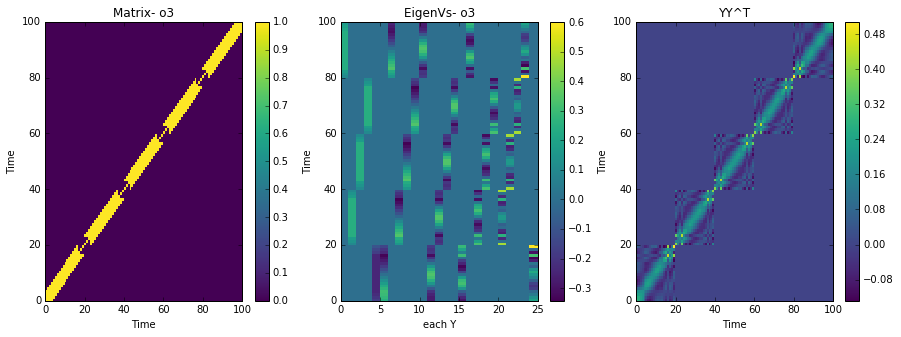
\includegraphics[width=0.8\textwidth]{./figure/o3_eachStage.png}
  \caption{The steps from symmetric matrix to eigenvector}
\end{figure}


\subsection{Boundary Detection}
As the pseudocode in Algorithm 2, once the Laplacian matrix is constructed, each row is the representation of eigen-features at specific time. Therefore, running k-means for eigen-features of all time points will yield the results of which centroids of this time point belongs to, and therefore the place where the $t_{i} \neq t_{i+1}$ is where the boundary is. As showed in figure 3.3, boundary is correctly detected at each time point, but when doing experiments I noticed the number of iteration during k-means will affect the correctness of boundary, and the more iteration usually gives better boundary.
\begin{figure}[H]
\centering
\begin{subfigure}
  \begin{tabular}{c}
  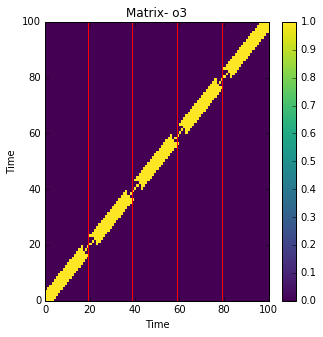
\includegraphics[width=25mm]{./figure/o3_boundary.png}
  \end{tabular}{}
\end{subfigure}
  \begin{tabular}{c}
  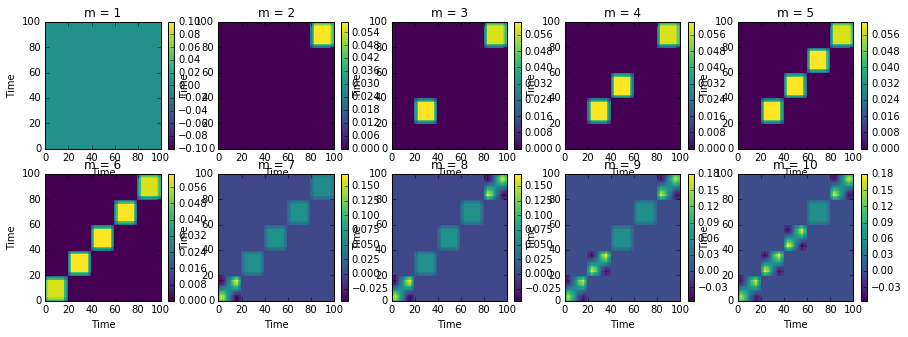
\includegraphics[width=75mm]{./figure/o3_eachM.png}
  \end{tabular}{}
\begin{subfigure}
\end{subfigure}
\caption{Boundary detection and pair-wise frame similarities ($YY^T$). Left: Boundary detection of original recurrence graph, and Right: visualization of $YY^T$ using the first 10 eigenvectors}
\end{figure}

\begin{algorithm}[htb]
  \caption{boundaryDetection}
  \SetKwInOut{Input: }{Laplacian eigenvectors $Y \in \mathbb{R^{n \times m}}$}

  \SetKwInOut{Output: }{Boundary b, Centroids c}
  \label{algo:SC}
\begin{algorithmic}[1]
  \STATE $ \overline y_i = \frac{Y_i}{\parallel Y \parallel}$ //normalize each row $Y_i$
  \STATE Run k-means on $\{ \overline y_i \}_{i=1}^{n}$
  \STATE Let $c_i$ denote the cluster containing $ \overline y_i$
  \STATE $b \leftarrow \{ i|c_i \neq c_{i+1}\}$
  \STATE return b, c
\end{algorithmic}
\end{algorithm}

\subsection{Affinity Matrix from Real Music}
As basic process is established above, I started to construct matrix from real music, and the music I started with is \textit{The Beatles - Come Together}. Data is sampled in the rate of 22050Hz, and transformed to .wav format, as it can be imported by scipy. Imported signal has two track, and all following analysis is based on the first track, and feature extraction is done by librosa cqt computing the constant-Q transform of an audio signal. As we get too little information at low frequencies and too much information at highfrequencies if we just simply double the frequency for Fourier transformation[Ref 6], and cqt will be better suit for extracting feature from music signal because it spaced the center frequencies of the frequency bins geometrically, and all Q-factors are all equal[Ref 7]. The \textit{ affinity matrix A} is constructed by:
\begin{equation}
A_{ij} = \mu R^{\prime}_{ij}S^{rep}_{ij} + (1-\mu)\Delta_{ij}S^{loc}_{ij}
\end{equation}
where $R_{ij}$ is recurrence matrix and $R[i][j]$ is 1 if time $i$ and $j$ are mutual k-nearest neighbors else is 0, and $R$ is symmetric. $\Delta[i][j]$ is 1 if $|i-j|=1$ else is 0. $S_{ij}$ is the result of matrix passed to $Gaussian Kernel$ of feature vectors $x_i$, $x_j$:
\begin{equation}
G(M) = S_{ij} = exp\left( {-1\over2\sigma^2} \|x_i-x_j\|^2  \right) \textbf{, for each row of i and j in M}
\end{equation}
and $S^{rep}_{ij} = G(R^{\prime}_{ij})$ and $S^{loc}_{ij} = G(\Delta_{ij})$, and $\mu$ is Equation 3.2 is a factor balancing local and global linkage, and optimal of $\mu$ is solved by:
\begin{equation}
\mu^{\ast} = {<d(\delta), d(R^{\prime})+d(\delta) >\over \|d(r^{\prime})+d(\delta)\|^2}
\end{equation}
where we treat the input matrix as vector of degree-sum where $d(\cdot)=[d_i(\cdot)]^n_{i=1}$, and $d_i(G) = \Sigma_jG_{ij}$ is the degree sum at time $i$. However, after the $affinity matrix A$ being constructed from Equation 3.2, we loss the symmetric proerity, eventhough R^{\prime}_{ij}, S^{rep}_{ij}, \Delta_{ij}, and S^{loc}_{ij} are symmetric. The dot product from Equation 3.2 is not symmetric, and there the addition modification may be required.


\begin{thebibliography}{10}
\bibitem{fpf} {\sc A Tutorial on Spectral Clustering}
\bibitem{fpf} {\sc Analyzing Song Structure with Spectral Clustering}
\bibitem{fpf} {\sc Deep clustering: Discriminative embeddings for
segmentation and separation}
\bibitem{fpf} {\sc Learning Deep Representations for Graph Clustering}
\bibitem{fpf} {\sc Hierarchical Evaluation of Segment Boundary Detection}
\bibitem{fpf} {\sc Calculation of a Constant Q Spectral Transformation}
\bibitem{fpf} {\sc Constant-Q Transform Toolbox for Music Processing}
\end{thebibliography}

\end{document}
